% GNUPLOT: LaTeX picture with Postscript
\begingroup
  \makeatletter
  \providecommand\color[2][]{%
    \GenericError{(gnuplot) \space\space\space\@spaces}{%
      Package color not loaded in conjunction with
      terminal option `colourtext'%
    }{See the gnuplot documentation for explanation.%
    }{Either use 'blacktext' in gnuplot or load the package
      color.sty in LaTeX.}%
    \renewcommand\color[2][]{}%
  }%
  \providecommand\includegraphics[2][]{%
    \GenericError{(gnuplot) \space\space\space\@spaces}{%
      Package graphicx or graphics not loaded%
    }{See the gnuplot documentation for explanation.%
    }{The gnuplot epslatex terminal needs graphicx.sty or graphics.sty.}%
    \renewcommand\includegraphics[2][]{}%
  }%
  \providecommand\rotatebox[2]{#2}%
  \@ifundefined{ifGPcolor}{%
    \newif\ifGPcolor
    \GPcolorfalse
  }{}%
  \@ifundefined{ifGPblacktext}{%
    \newif\ifGPblacktext
    \GPblacktexttrue
  }{}%
  % define a \g@addto@macro without @ in the name:
  \let\gplgaddtomacro\g@addto@macro
  % define empty templates for all commands taking text:
  \gdef\gplbacktext{}%
  \gdef\gplfronttext{}%
  \makeatother
  \ifGPblacktext
    % no textcolor at all
    \def\colorrgb#1{}%
    \def\colorgray#1{}%
  \else
    % gray or color?
    \ifGPcolor
      \def\colorrgb#1{\color[rgb]{#1}}%
      \def\colorgray#1{\color[gray]{#1}}%
      \expandafter\def\csname LTw\endcsname{\color{white}}%
      \expandafter\def\csname LTb\endcsname{\color{black}}%
      \expandafter\def\csname LTa\endcsname{\color{black}}%
      \expandafter\def\csname LT0\endcsname{\color[rgb]{1,0,0}}%
      \expandafter\def\csname LT1\endcsname{\color[rgb]{0,1,0}}%
      \expandafter\def\csname LT2\endcsname{\color[rgb]{0,0,1}}%
      \expandafter\def\csname LT3\endcsname{\color[rgb]{1,0,1}}%
      \expandafter\def\csname LT4\endcsname{\color[rgb]{0,1,1}}%
      \expandafter\def\csname LT5\endcsname{\color[rgb]{1,1,0}}%
      \expandafter\def\csname LT6\endcsname{\color[rgb]{0,0,0}}%
      \expandafter\def\csname LT7\endcsname{\color[rgb]{1,0.3,0}}%
      \expandafter\def\csname LT8\endcsname{\color[rgb]{0.5,0.5,0.5}}%
    \else
      % gray
      \def\colorrgb#1{\color{black}}%
      \def\colorgray#1{\color[gray]{#1}}%
      \expandafter\def\csname LTw\endcsname{\color{white}}%
      \expandafter\def\csname LTb\endcsname{\color{black}}%
      \expandafter\def\csname LTa\endcsname{\color{black}}%
      \expandafter\def\csname LT0\endcsname{\color{black}}%
      \expandafter\def\csname LT1\endcsname{\color{black}}%
      \expandafter\def\csname LT2\endcsname{\color{black}}%
      \expandafter\def\csname LT3\endcsname{\color{black}}%
      \expandafter\def\csname LT4\endcsname{\color{black}}%
      \expandafter\def\csname LT5\endcsname{\color{black}}%
      \expandafter\def\csname LT6\endcsname{\color{black}}%
      \expandafter\def\csname LT7\endcsname{\color{black}}%
      \expandafter\def\csname LT8\endcsname{\color{black}}%
    \fi
  \fi
    \setlength{\unitlength}{0.0500bp}%
    \ifx\gptboxheight\undefined%
      \newlength{\gptboxheight}%
      \newlength{\gptboxwidth}%
      \newsavebox{\gptboxtext}%
    \fi%
    \setlength{\fboxrule}{0.5pt}%
    \setlength{\fboxsep}{1pt}%
    \definecolor{tbcol}{rgb}{1,1,1}%
\begin{picture}(4320.00,3744.00)%
    \gplgaddtomacro\gplbacktext{%
      \csname LTb\endcsname%%
      \put(84,748){\makebox(0,0)[r]{\strut{}$0$}}%
      \put(84,1149){\makebox(0,0)[r]{\strut{}$0.1$}}%
      \put(84,1550){\makebox(0,0)[r]{\strut{}$0.2$}}%
      \put(84,1951){\makebox(0,0)[r]{\strut{}$0.3$}}%
      \put(84,2352){\makebox(0,0)[r]{\strut{}$0.4$}}%
      \put(84,2753){\makebox(0,0)[r]{\strut{}$0.5$}}%
      \put(84,3154){\makebox(0,0)[r]{\strut{}$0.6$}}%
      \put(84,3555){\makebox(0,0)[r]{\strut{}$0.7$}}%
      \put(216,528){\makebox(0,0){\strut{}$50$}}%
      \put(702,528){\makebox(0,0){\strut{}$51$}}%
      \put(1188,528){\makebox(0,0){\strut{}$52$}}%
      \put(1674,528){\makebox(0,0){\strut{}$53$}}%
      \put(2160,528){\makebox(0,0){\strut{}$54$}}%
      \put(2645,528){\makebox(0,0){\strut{}$55$}}%
      \put(3131,528){\makebox(0,0){\strut{}$56$}}%
      \put(3617,528){\makebox(0,0){\strut{}$57$}}%
      \put(4103,528){\makebox(0,0){\strut{}$58$}}%
      \put(2766,1237){\makebox(0,0)[l]{\strut{}$(\varphi_B, 0.032)$}}%
    }%
    \gplgaddtomacro\gplfronttext{%
      \csname LTb\endcsname%%
      \put(-521,2151){\rotatebox{-270.00}{\makebox(0,0){\strut{}U (mV)}}}%
      \put(2159,198){\makebox(0,0){\strut{}úhel dopadu $\varphi$ (°)}}%
    }%
    \gplbacktext
    \put(0,0){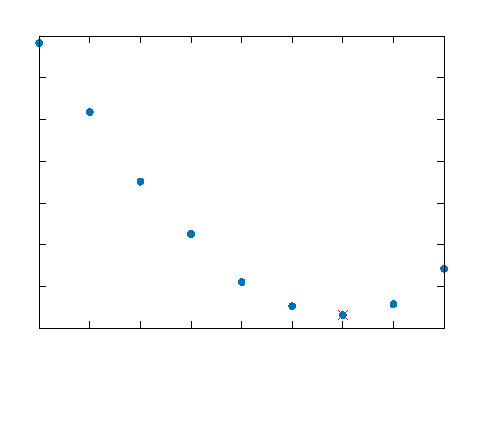
\includegraphics[width={216.00bp},height={187.20bp}]{brewster_uhel}}%
    \gplfronttext
  \end{picture}%
\endgroup
